% File: ot-lca.tex
\documentclass{standalone}

\usepackage{amssymb}
\usepackage{tikz}
\usetikzlibrary{shapes, positioning, arrows.meta, calc, backgrounds, fit, decorations.pathmorphing}

\newcommand{\state}[3]{% #1: state name; #2: position; #3: state label
  \node (#1) [circle, inner sep = 0pt, minimum size = 8mm, text width = 8mm, align = center, draw, #2, font = \Large] {#3};
}

\tikzset{path/.style = {>=Stealth, ->, decorate, decoration = {snake, post length = 1mm}}}
\tikzset{edge/.style = {>=Stealth, ->}}

\begin{document}
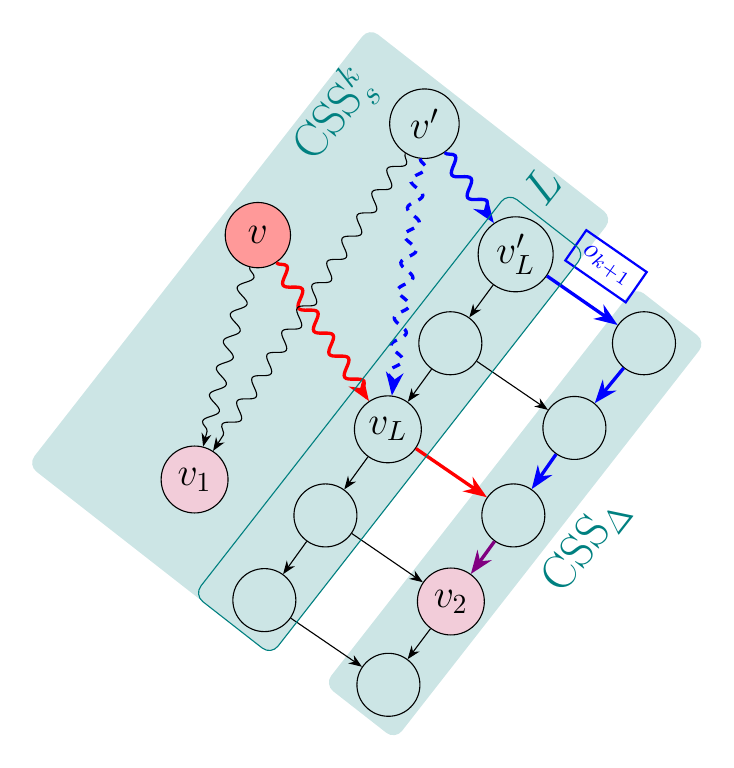
\begin{tikzpicture}[p1/.style = {red, very thick},
	p2/.style = {blue, very thick}]
  \state{s}{fill = red!40}{$v$}
  \state{s'}{above right = 0.8cm and 1.5cm of s}{$v'$}
  \state{s1}{below left = 2.5cm and 0.2cm of s, fill = purple!20}{$v_1$}

  \state{sl'}{below right = 1.0cm and 0.5cm of s'}{$v'_{L}$}
  \state{sx}{below left = 0.5cm and 0.2cm of sl'}{}
  \state{sy}{below left = 0.5cm and 0.2cm of sx}{$v_{L}$}
  \state{sz}{below left = 0.5cm and 0.2cm of sy}{}
  \state{sf}{below left = 0.5cm and 0.2cm of sz}{}
  \draw[edge] (sl') to (sx);
  \draw[edge] (sx) to (sy);
  \draw[edge] (sy) to (sz);
  \draw[edge] (sz) to (sf);

  \state{sl''}{below right = 0.5cm and 1.0cm of sl'}{}
  \state{sx'}{below right = 0.5cm and 1.0cm of sx}{}
  \state{sy'}{below right = 0.5cm and 1.0cm of sy}{}
  \state{sz'}{below right = 0.5cm and 1.0cm of sz, fill = purple!20}{$v_2$}
  \state{sf'}{below right = 0.5cm and 1.0cm of sf}{}
  \draw[edge, p2] (sl'') to (sx');
  \draw[edge, p2] (sx') to (sy');
  \draw[edge, very thick, red!50!blue] (sy') to (sz');
  \draw[edge] (sz') to (sf');

  \draw[edge, p2] (sl') to node[above = 8pt, rectangle, draw, thick, sloped] {$o_{k+1}$} (sl'');
  \draw[edge] (sx) to (sx');
  \draw[edge, p1] (sy) to (sy');
  \draw[edge] (sz) to (sz');
  \draw[edge] (sf) to (sf');

  \draw[path] (s) to (s1);
  \draw[path, p1] (s) to (sy);

  \draw[path] (s') to (s1);
  \draw[path, p2] (s') to (sl');

  \draw[path, p2, dashed] (s') to (sy);

	\node () [rectangle, rounded corners, inner sep = 5pt, rotate fit = 52, 
	  draw = teal,
	  fit = (sl') (sx) (sf), 
	  label = {[rotate = 52, font = \LARGE, teal]0:$L$}] {};

  \begin{pgfonlayer}{background}
	\node () [rectangle, rounded corners, inner sep = 5pt, rotate fit = 52, 
	  fill = teal!20,
	  fit = (s) (s') (s1) (sl') (sx) (sf), 
	  label = {[rotate = 52, font = \LARGE, label distance = -0.8cm, teal]40:CSS$_{s}^{k}$}] {};
  \end{pgfonlayer}

  \begin{pgfonlayer}{background}
	\node () [rectangle, rounded corners, inner sep = 5pt, rotate fit = 52, 
	  fill = teal!20,
	  fit = (sl'') (sx') (sy') (sz') (sf'), 
	  label = {[rotate = 52, font = \LARGE, teal]-135:CSS$_{\Delta}$}] {};
  \end{pgfonlayer}
\end{tikzpicture}
\end{document}
